It is important to get a sense of how the area of nonlinear dynamics has been applied to neuroscience.
One of the most powerful tools for describing the qualitative behavior of a nonlinear system is \textit{bifurcation analysis}, determining how the number and stability of fixed points and limit cycles changes as parameters of a model change \cite{Strogatz2015}.
\section{Bifurcation Analyses of Seizure Models}
\label{sec:lit_review_bifurcation}
Analyses of the dynamics of brain models can provide an understanding of the mechanisms underlying a wide variety of brain behaviors.
Multistability and bifurcations can be interpreted as being at the center of many different states, from seizures to switching from syncopated to anti-syncopated finger tapping [\onlinecite{Wang2012,Jirsa2014,Santos2017,Baier2012,Breakspear2005,Jirsa2014,Breakspear2017}].
In this section, we review some examples of bifurcation analyses of neural models.
\subsubsection{The Wilson-Cowan Model}
\label{sec:lit_review_bifurcation_wc}
One of the simplest models which lends itself to bifurcation analysis is the Wilson-Cowan model (\cref{eq:wc_x,eq:wc_y,eq:wc_z}).
Traces of $x$ over time look remarkably like the output from an EEG scan.
\Cref{fig:wc_and_swe} shows a simulation of the Wilson-Cowan model with the parameters\footnote{Parameters taken from [\onlinecite{Wang2012}], table 1.  Note that the values in rows 3(g),3(i) and 3(j),3(l) should be switched.}:
\begin{equation*}
  \label{eq:wc_params}
  C
  =
  \bmqty{23 & -15 & -10 \\ 35 & 0 & 0 \\ 10 & 0 & 0}
  \qc
  \bmqty{P \\ Q \\ R}
  =
  \bmqty{3 \\ -5 \\ -5}, \\
\end{equation*}
and
\begin{equation}
  \tau
  =
  \bmqty{0.015 \\ 0.013 \\ 0.267}.
\end{equation}
These results show a stereotypical spike-wave event, represented to a high degree of accuracy relative to the simplicity of the model.
\begin{figure}[ht]
  \centering
  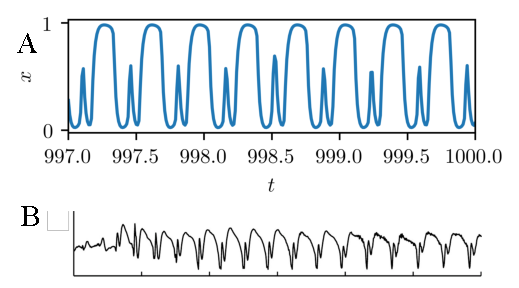
\includegraphics[width=\columnwidth]{figure/wc.pdf}
  \caption[Wilson-Cowan simulation and spike-wave event]{A comparison of a simulation of the Wilson-Cowan system and an actual EEG trace of spike-wave event.
    A. The output of a simulation of the Wilson-Cowan model (\cref{eq:wc_x,eq:wc_y,eq:wc_z}) using parameters from [\onlinecite{Wang2012}].
    We ran a 4th-order Runge-Kutta solver ($\dd{t} = 0.01$, $t_{\text{max}} = 1000$) on the Wilson-Cowan model with parameters shown in \cref{eq:wc_params}.
    B. An EEG trace of a spike-wave event, often characteristic of absence seizures.
    Taken and modified from [\onlinecite{Marten2009}].
  }
  \label{fig:wc_and_swe}
\end{figure}

The main challenge for performing bifurcation analysis on this type of system is two-fold.
The first aspect is that there are 15 parameters to vary.
This makes bifurcation analysis exceedingly difficult, as all 15 dimensions and their relationships to each other must be analyzed.
This is closely related to the second aspect of the challenge this model provides: the variables in this model are abstracted from their physical/physiological meanings.
For example, because the coupling strengths do not correspond directly to any measurable values, it is hard to gain actionable semantic knowledge from analysis of their effects on the system [\onlinecite{Jirsa2014}].

However, it is possible to observe a bifurcation if the external input $P$ varies (\cref{eq:wc_x}).
\Cref{fig:wc_bifurcation} shows the change from spike-wave behavior to simple wave behavior as $P$ increases past 3.92, at time 47.3.
While it would be impossible to do an exhaustive sweep of parameter space, one can in principle observe all of the dynamics of brain behavior in this model.
\begin{figure}[ht]
  \centering
  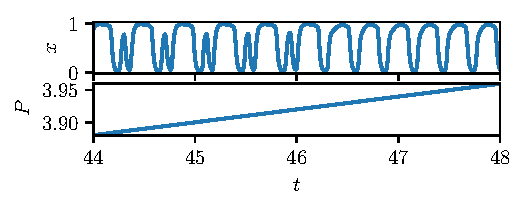
\includegraphics[width=\columnwidth]{figure/wc_bifurcation.pdf}
  \caption[Wilson-Cowan bifurcation]{A bifurcation from spike-wave behavior to simple wave behavior in the Wilson-Cowan model as a function of continuously varying external input parameter $P$.
    For the simulation, we used a 4th-order Runge-Kutta solver ($\dd{t} = 0.01$, $t_{max} = 100$) as $P$ linearly increased from 3 to 5.
  }
  \label{fig:wc_bifurcation}
\end{figure}

\subsubsection{The Epileptor Model}
\label{sec:lit_review_bifurcation_epileptor}
In the Epileptor model (\cref{eq:epileptor_x1,eq:epileptor_y1,eq:epileptor_z,eq:epileptor_x2,eq:epileptor_y2,eq:epileptor_f1,eq:epileptor_f2,eq:epileptor_g}), bifurcations depending on the slow permittivity variable $z$ determine whether the brain is behaving normally, or having a seizure [\onlinecite{Jirsa2014}].
Given the time scale on which $z$ varies ($\frac{1}{2857}$ times as fast as $x_{1}$) and the bifurcations' dependence on it, $z$ acts like an external parameter to the system, causing the model to go into and out of seizure.
In \cref{fig:epileptor}, the transitions into and out of seizure are clear as critical points in $z$.
In particular, as is the case with many similar models, normal steady-state brain function corresponds to a stable fixed point, while seizure-like events are represented by stable limit cycles.
This raises a question: what kinds of bifurcations occur during the transition from healthy brain activity to seizures and back?
\begin{figure}[ht]
  \centering
  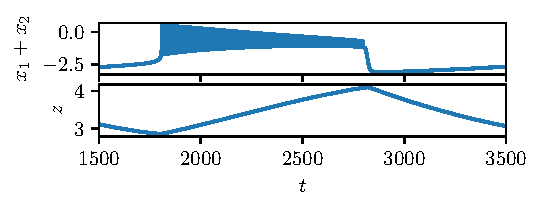
\includegraphics[width=\columnwidth]{figure/epileptor.pdf}
  \caption[Epileptor simulation]{A simulation of the Epileptor model showing the observable $x_{1}$ and the slow-changing permittivity variable $z$, using a 4th-order Runge-Kutta solver ($\dd{t} = 0.01$, $t_{\text{max}} = 2000$) and the parameters listed in \cref{sec:intro_seizures_aetiology}.
    The brain is exhibiting healthy behavior for $t \in \pqty{0, 360} = h_{1}$, then rapidly jumps into a seizure-like behavior.
    It stays in this state for $t \in \pqty{360, 1360} = s$, until it returns to a healthy fixed point for $t \in \pqty{1360, 2000} = h_{2}$.
    Note the DC shift, wherein $x_{1}(s) > x_{1}(h_{1}) \approx x_{1}(h_{2})$.
  }
  \label{fig:epileptor}
\end{figure}

To discuss the dynamics of Epileptor in general, we will use the stereotypical behavior displayed in \cref{fig:epileptor}.
An important aspect of Epileptor to note is that $x_{1} + x_{2}$ is the closest variable to an observable quantity, but it still does not resemble an EEG trace without some post-processing.
For example, $x_{1}$ would look a lot more like the output from an EEG if put through a high-pass filter.
However, there is an invertible map directly between $x_{1} + x_{2}$ and the readings from an EEG, so the results can be treated as the same [\onlinecite{Jirsa2014}].

During seizure onset at $t = 360$, the stable fixed point of healthy activity disappears, replaced by a stable limit cycle.
This indicates that the system undergoes either a Hopf or a saddle-node bifurcation.
A hint towards the type of bifurcation involved is that seizures occur suddenly [\onlinecite{Kandel2013}].
This means that the amplitude of oscillation does not steadily increase from 0, meaning that a supercritical Hopf bifurcation can be ruled out [\onlinecite{Strogatz2015}].
At $t = 360$, the mean values of $x_{1} + x_{2}$ jump from $\expval{x_{1}(t) + x_{2}(t)}_{t \in h_{1}} = -2.5$ to $\expval{x_{1}(t) + x_{2}(t)}_{t \in s} = -0.8$.
This DC shift does appear in experiment, and indicates that the bifurcation can not be a subcritical Hopf.
This leaves only a saddle-node bifurcation for the transition into a seizure [\onlinecite{Jirsa2014}].

As the seizure ends at $t = 1360$, the model returns from a limit cycle to a fixed point with another DC shift.
This indicates that the bifurcation is either a fold bifurcation or a homoclinic bifurcation.
One important point of note is that the frequency of oscillation decreases as the seizure approaches offset, which matches with experiment.
This indicates that the transition must be a homoclinic bifurcation, because systems maintain constant frequency as they approach fold bifurcations [\onlinecite{Jirsa2014}].

%%% Local Variables:
%%% mode: latex
%%% TeX-master: "../../ms"
%%% End:



\section{Chimera States in the Brain}
\label{sec:lit_review_chimera}
We show the normalized chimera-like index of the entire physical region in \cref{fig:aphysical_chimera}.
Near the maximal edge of the physical region, the highest values of the chimera index appear to follow a slope of $-1$.
It is unsurprising that chimera states would be prevalent when the coupling is large (out near the boundary of the aphysical range).

What is surprising, however, is the presence of the chimeric patch in the bottom left corner of \cref{fig:aphysical_chimera}, shown at a higher resolution in \cref{fig:zoom}.
\begin{figure}[ht]
  \centering
  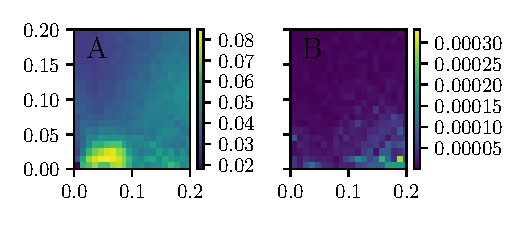
\includegraphics[width=0.5\textwidth]{figure/zoom_100dpi.pdf}
  \caption[Zoomed landscape]{A.\ The chimera-like index $\chimera$ of runs with $(\hra, \hrb) \in (0, 0.2) \times (0, 0.2)$.
    As before, the chimera-like index is normalized to $\frac{1}{7}$.
    Note that the values of the index are much higher in this patch than in most of the rest of $(\hra, \hrb) \in (0, 1) \times (0, 1)$ (\cref{fig:aphysical_chimera}).
    B.\ The variance of the chimera-like index.
  }
  \label{fig:zoom}
\end{figure}
Plotting the results of the simulations (\cref{fig:041_021}),
it is evident that this is not a calculation error, but is an actual feature of the parameter landscape.
\begin{figure*}[ht]
  \centering
  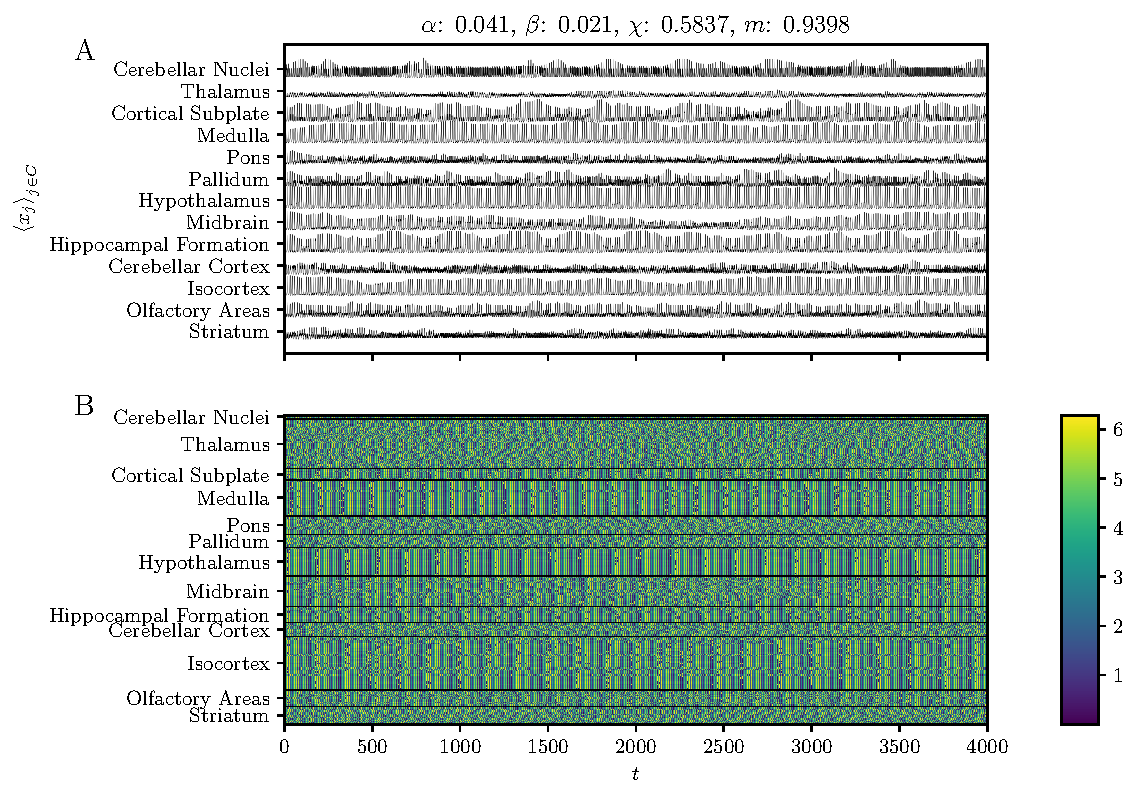
\includegraphics[width=\textwidth]{figure/0_041-0_021_200dpi.pdf}
  \caption[Highly chimeric simulation]{A run of the Hindmarsh-Rose simulation in the chimeric island.
    A. The mean membrane potential within each cortex.
    B. The phase $\phase$ of the entire timeseries for a simulation of the Hindmarsh-Rose network.
    Synchronization is most consistently evident in the medulla, the hypothalamus, and the isocortex.
  }
  \label{fig:041_021}
\end{figure*}

The highly chimeric patch within the physical portion of the landscape appears to be mostly below the $\beta = \alpha$ line.
This is reasonable, as chimera states occur when coupling within groups is greater than coupling between groups.
A small portion of the chimeric patch lies above the $\beta = \alpha$ line, likely because the average strength between cortices is greater than the average strength within cortices (see \cref{fig:average_strengths} A).

The chimera-like index $\chimera$ greatly lessens at $\alpha \approx 0.1$.
A possible explanation for this comes from comparing the order of $\dot{\hrx}$ without the coupling terms, and the coupling terms themselves.
From our simulation, we find that $\dot{\hrx}$ without the coupling terms ranges roughly from -6 to 3.
The coupling terms each\footnote{Since the same can be said for both $\alpha$ and $\beta$, we will discuss only $\alpha$, with the understanding that $\beta$ could be substituted into the proceeding sentences.}
range from 0 to approximately $30 \alpha$.
This means that, when $\alpha > 0.1$, the coupling is at least of the same order as the sum of the rest of the terms in the equation.
This leads to a qualitative difference between the two states, which likely manifests itself as the less-chimeric states.

%%% Local Variables:
%%% mode: latex
%%% TeX-master: "../../ms"
%%% End:

